\documentclass[runningheads]{llncs}

\usepackage[T1]{fontenc}
\usepackage{graphicx}
\usepackage{amsmath,amssymb}
\usepackage{booktabs}
\usepackage{tikz}
\usetikzlibrary{positioning,arrows.meta,fit}
\usepackage{xcolor}
\usepackage{marvosym}
\usepackage{hyperref}
\hypersetup{colorlinks=true,linkcolor=blue,citecolor=blue,urlcolor=blue}

\begin{document}

\title{StepWise: An Explainable Classical Machine Learning Tutor for Diagnosing Misconceptions in Handwritten Mathematics}
\titlerunning{StepWise: Explainable ML Tutoring for Handwritten Mathematics}

\author{Siddhi J Salunkhe \and Sanvi Saket \and Prof. Manjula R}
\authorrunning{S. J. Salunkhe et al.}

\institute{Department of Computer Science and Engineering, Vellore Institute of Technology,\\ Vellore, Tamil Nadu, India}

\maketitle

\begin{abstract}
Students make systematic, repeatable mistakes in arithmetic and early algebra, but teachers rarely have time to give individual feedback on handwritten work. Existing tools either solve the problem for the student or rely on large neural and language models that are opaque, costly and can state mathematically wrong explanations. We present StepWise, an explainable tutoring system that reads a photograph of handwritten working, proves which step is wrong, names the likely misconception and recommends targeted practice, using only classical machine learning. Handwritten symbols are segmented with OpenCV and classified by a support vector machine on histogram-of-oriented-gradient features; every step is verified exactly with SymPy; a random forest over 33 interpretable features classifies the misconception; a second classifier trained on 1,720 real student mistakes separates careless slips from understanding gaps; and Bayesian knowledge tracing with item response theory drives adaptive practice. On the official CROHME 2014/2016/2019 test sets (unseen writers) the recognizer reaches 92.4\% symbol accuracy (95\% CI 91.2--93.6\%), against 55.4\% when trained on fonts only, and reads whole expressions twice as often as a zero-shot transformer OCR baseline (56.7\% vs.\ 28.4\% exact match, $p<10^{-6}$) while being 28 times faster and 160 times smaller. An illumination-normalisation step raises accuracy under uneven lighting from 3.1\% to 56.7\%. On ScratchMath, a classifier trained on 1,720 real student mistakes separates careless slips from understanding gaps with 68.3\% accuracy against a 55.2\% majority baseline ($p<0.001$), and on ASSISTments 2009 (446,844 real answers) knowledge tracing predicts the next answer with an AUC of 0.815. The full system runs offline on a laptop CPU.

\keywords{Intelligent tutoring \and Handwritten mathematics \and Misconception diagnosis \and Support vector machine \and Knowledge tracing \and Explainable AI.}
\end{abstract}

%% ------------------------------------------------------------------
\section{Introduction}

Arithmetic and early algebra errors are rarely random. A student who writes $-3+5=-8$ or moves $+4$ across the equals sign without changing its sign is usually following a consistent but faulty procedure, a ``bug'' in the sense of Brown and Burton~\cite{brown1978}. Diagnosing these bugs early is valuable because each one can be repaired with a short, targeted explanation. In practice, however, a teacher marking a class set of handwritten worksheets can only mark answers right or wrong; the information about \emph{why} an answer is wrong stays on the page.

Software can help, but current tools address a different problem. Photo-solver applications recognise a printed problem and return the solution, which removes the need for the student to think. Intelligent tutoring systems such as Cognitive Tutor~\cite{koedinger1997} diagnose errors well but require typed, step-by-step input in a dedicated interface. Recent approaches based on deep networks and large language models can read handwriting and generate explanations, but they need GPUs or paid APIs, are hard to audit, and can confidently state incorrect mathematics~\cite{song2026scratchmath}.

This paper presents StepWise, a tutoring system built around three design decisions. First, \emph{exact mathematics is used wherever truth can be proved}: every line of the student's working is verified symbolically, so the system never invents an error. Second, \emph{classical machine learning is used wherever there is genuine uncertainty}: reading handwriting, deciding which kind of mistake was made, estimating mastery and grouping students. Third, \emph{every learned component is evaluated on real, publicly available data} with baselines and held-out test sets. The main contributions are:
\begin{itemize}
\item an end-to-end pipeline from a photograph of handwritten working to a verified, explained misconception diagnosis and adaptive practice, running offline on a CPU;
\item a learned ``bug library'': classical misconception rules turned into 33 named features for a random forest, so that each diagnosis is accompanied by the evidence that produced it;
\item a count-alignment procedure that harvests labelled real handwritten symbols from CROHME expression-level annotations, and an evaluation showing that training on real handwriting raises symbol accuracy on unseen writers from 55.4\% to 92.4\%;
\item a head-to-head comparison with a transformer OCR model on the same real test expressions, and a robustness study under simulated phone-photo conditions with an illumination-normalisation step;
\item an evaluation of knowledge tracing on ASSISTments 2009 and of a slip-versus-understanding classifier on ScratchMath, the only public dataset of real handwritten student mistakes with error labels that we are aware of, with bootstrap confidence intervals, significance tests and feature ablations.
\end{itemize}

%% ------------------------------------------------------------------
\section{Related Works}

\textbf{Diagnosing procedural errors.} Brown and Burton~\cite{brown1978} modelled students' subtraction errors as ``bugs'' in otherwise correct procedures and built a library of such bugs to explain wrong answers. VanLehn~\cite{vanlehn1990} extended this into a theory of how bugs arise. Model-tracing tutors~\cite{koedinger1997} follow each typed step and match it against correct and buggy production rules. StepWise keeps the idea of a bug library but encodes each bug as a feature and lets a classifier learn how to weigh overlapping evidence, instead of relying on hand-ordered rules.

\textbf{Handwritten mathematical expression recognition.} The CROHME competitions~\cite{mouchere2014,mahdavi2019} established the standard benchmark for handwritten mathematical expressions. Recent systems are encoder--decoder neural networks such as WAP~\cite{zhang2017wap} and transformer-based OCR such as TrOCR~\cite{li2023trocr}. These achieve high accuracy on full two-dimensional expressions but require GPU training and large models. For isolated characters, histogram-of-oriented-gradient (HOG) features~\cite{dalal2005} with support vector machines~\cite{cortes1995} remain a strong and efficient baseline~\cite{maji2009}; the HASYv2 dataset~\cite{thoma2017} provides real handwritten symbols from many writers.

\textbf{Knowledge tracing.} Bayesian Knowledge Tracing (BKT)~\cite{corbett1994} models each skill as a hidden learned/unlearned state. Performance Factors Analysis (PFA)~\cite{pavlik2009} instead uses logistic regression on counts of past successes and failures. Deep Knowledge Tracing~\cite{piech2015} uses recurrent networks, although later work showed that well-specified classical models remain competitive~\cite{xiong2016}. Item response theory~\cite{rasch1960} estimates item difficulty and learner ability. ASSISTments~\cite{feng2009} provides the most widely used public benchmark.

\textbf{Datasets of student mistakes.} Public data on \emph{why} students err is scarce. ScratchMath~\cite{song2026scratchmath} provides real handwritten scratchwork from primary and middle-school students with expert error categories; its authors show that even multimodal large language models struggle to identify the error type. StepWise is, to the best of our knowledge, the first system to combine symbolic step verification, classical misconception classification and knowledge tracing in one offline pipeline evaluated on these real datasets.

%% ------------------------------------------------------------------
\section{Dataset}

Table~\ref{tab:datasets} lists the datasets. All real datasets are downloaded from their public sources by a script and are never redistributed with the code.

\begin{table}[t]
\caption{Datasets used in this work.}\label{tab:datasets}
\centering\scriptsize
\begin{tabular}{@{}p{2.6cm}p{1.2cm}p{3.6cm}p{3.6cm}@{}}
\toprule
Dataset & Type & Size used & Purpose \\
\midrule
CROHME train~\cite{mouchere2014} & real & 6,271 symbols from 1,337 expressions & symbol recognizer training \\
CROHME 2014/16/19 test~\cite{mahdavi2019} & real & 1,821 symbols; 127 expressions & symbol and expression testing (unseen writers) \\
HASYv2~\cite{thoma2017} & real & 3,335 symbols, 144 writers & symbol recognizer training \\
ASSISTments 2009~\cite{feng2009} & real & 446,844 answers, 4,151 students, 110 skills & knowledge tracing \\
ScratchMath~\cite{song2026scratchmath} & real & 1,720 wrong answers with scratchwork photos & error-type classifier \\
Font-rendered glyphs & synthetic & 12,210 glyphs from 24 fonts & robustness to printed input \\
Generated solutions & synthetic & 3,150 solutions, 9 classes & fine-grained misconception classifier \\
\bottomrule
\end{tabular}
\end{table}

\textbf{Harvesting real symbols from CROHME.} CROHME annotates whole expressions in \LaTeX{} but provides no symbol bounding boxes in the image release we use. We keep only \emph{linear} expressions (no fractions, scripts or roots), segment each with the same OpenCV segmenter used at inference time, and, when the number of segmented components equals the number of \LaTeX{} tokens, label the crops in left-to-right order. Expressions where the counts differ are discarded. Of 2,185 linear training expressions, 1,337 aligned, giving 6,271 labelled symbols over 17 classes (\texttt{0}--\texttt{9}, \texttt{+ - = x ( ) /}, with $\times$ mapped to \texttt{x}). A manual check of 80 random crops found 79 correctly labelled. Fig.~\ref{fig:crops} shows examples.

\begin{figure}[t]
\centering
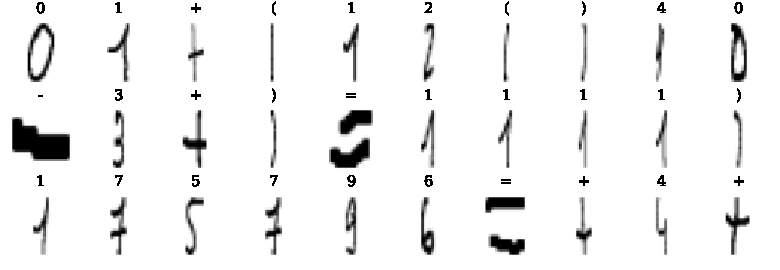
\includegraphics[width=0.85\textwidth]{figures/fig_aligned_crops.pdf}
\caption{A random sample of real handwritten symbols harvested from CROHME by count alignment, after size normalisation (labels above). Thick, blocky strokes are artifacts of the stretched CROHME renderings.}\label{fig:crops}
\end{figure}

\textbf{Real student mistakes.} ScratchMath contains 1,720 wrong answers from Chinese primary (1,479) and middle-school (241) students. Each record holds the question, the correct answer, a reference solution, the student's answer, a photograph of the student's handwritten scratchwork and one of seven expert error categories: calculation (566), question misunderstanding (519), concept (219), strategy (135), copying (124), reasoning (75) and attention (82). The expert's free-text explanation is never used as an input, because it reveals the label.

%% ------------------------------------------------------------------
\section{Methodology}

\subsection{System Overview}

Fig.~\ref{fig:arch} shows the pipeline. A photograph is cleaned and segmented, each symbol is classified, the recognised lines are verified symbolically, and the verified steps feed a misconception classifier. Its output drives feedback, mastery tracking, practice selection and the teacher's class view. Symbols the recognizer is unsure about are highlighted; when a student corrects one, the crop is stored as labelled training data for the next model version.

\begin{figure}[t]
\centering
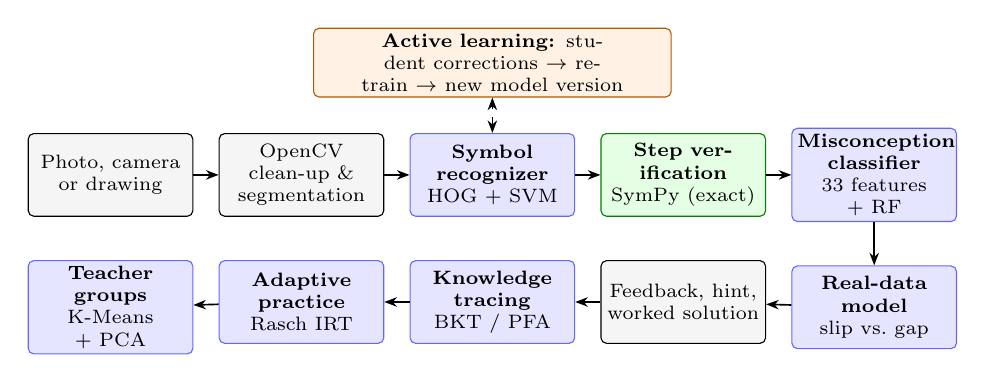
\begin{tikzpicture}[
  node distance=0.32cm and 0.32cm,
  box/.style={draw, rounded corners=2pt, align=center, font=\scriptsize, minimum height=1.05cm, text width=1.95cm, inner sep=2pt, fill=gray!8},
  ml/.style={box, fill=blue!10, draw=blue!60},
  ex/.style={box, fill=green!10, draw=green!50!black},
  arr/.style={-{Stealth[length=1.6mm]}, semithick}]
\node[box] (in) {Photo, camera or drawing};
\node[box, right=of in] (pre) {OpenCV clean-up \& segmentation};
\node[ml, right=of pre] (ocr) {\textbf{Symbol recognizer}\\HOG + SVM};
\node[ex, right=of ocr] (sym) {\textbf{Step verification}\\SymPy (exact)};
\node[ml, right=of sym] (mis) {\textbf{Misconception classifier}\\33 features + RF};
\node[ml, below=0.55cm of mis] (real) {\textbf{Real-data model}\\slip vs.\ gap};
\node[box, below=0.55cm of sym] (fb) {Feedback, hint, worked solution};
\node[ml, below=0.55cm of ocr] (kt) {\textbf{Knowledge tracing}\\BKT / PFA};
\node[ml, below=0.55cm of pre] (rec) {\textbf{Adaptive practice}\\Rasch IRT};
\node[ml, below=0.55cm of in] (clu) {\textbf{Teacher groups}\\K-Means + PCA};
\node[box, above=0.45cm of ocr, text width=4.4cm, minimum height=0.7cm, fill=orange!10, draw=orange!70!black] (al) {\textbf{Active learning:} student corrections $\rightarrow$ retrain $\rightarrow$ new model version};
\draw[arr] (in) -- (pre); \draw[arr] (pre) -- (ocr); \draw[arr] (ocr) -- (sym); \draw[arr] (sym) -- (mis);
\draw[arr] (mis) -- (real); \draw[arr] (real) -- (fb); \draw[arr] (fb) -- (kt); \draw[arr] (kt) -- (rec); \draw[arr] (rec) -- (clu);
\draw[arr, dashed, {Stealth[length=1.6mm]}-{Stealth[length=1.6mm]}] (ocr.north) -- (al.south);
\end{tikzpicture}
\caption{StepWise architecture. Blue boxes are learned components; the green box is exact symbolic computation.}\label{fig:arch}
\end{figure}

\subsection{Preprocessing and Segmentation}

The image is corrected for EXIF orientation and converted to greyscale. Photographs of paper are often unevenly lit, which breaks a global threshold, so the background is estimated and divided out before binarisation:
\begin{equation}
B=G_{\sigma}*\bigl(I\bullet E_k\bigr),\qquad I_{\text{norm}}=\min\!\Bigl(255,\;255\,\frac{I}{B}\Bigr),
\end{equation}
where $I\bullet E_k$ is a grey-level morphological closing with an elliptical element of size $k$ (about one twelfth of the shorter image side), which removes thin dark strokes and leaves the background, and $G_\sigma$ is a Gaussian blur. $I_{\text{norm}}$ is then binarised with Otsu's threshold. Text lines are found from the horizontal projection profile, and symbols within a line are the connected components of ink. Components whose horizontal extents overlap by at least half of the narrower one (the two bars of ``$=$'', a broken digit) are merged into one symbol. Spacing in the output is canonical rather than taken from the handwriting, and an \texttt{x} written between two numbers is interpreted as multiplication.

\subsection{Symbol Recognition}

Each symbol crop is scaled, preserving its aspect ratio, into a $28\times28$ canvas. For each pixel, the gradient magnitude and orientation are
\begin{equation}
m(u,v)=\sqrt{G_x(u,v)^2+G_y(u,v)^2},\qquad \theta(u,v)=\operatorname{atan2}\bigl(G_y(u,v),G_x(u,v)\bigr),
\end{equation}
and HOG features~\cite{dalal2005} accumulate $m$ into 9 orientation bins over $7\times7$-pixel cells grouped into overlapping blocks (324 values). These are concatenated with a $7\times7$ grid of ink densities (49 values) and the log aspect ratio of the bounding box (1 value), giving a 374-dimensional vector $\mathbf{x}$. A one-versus-one support vector machine~\cite{cortes1995} with the radial basis kernel classifies the symbol:
\begin{equation}
f(\mathbf{x})=\operatorname{sign}\Bigl(\sum_{i}\alpha_i y_i\,K(\mathbf{x}_i,\mathbf{x})+b\Bigr),\qquad K(\mathbf{x},\mathbf{x}')=\exp\bigl(-\gamma\lVert\mathbf{x}-\mathbf{x}'\rVert^2\bigr).
\end{equation}
Platt-scaled probabilities give a confidence for each symbol and its runner-up alternatives, which the interface uses to highlight symbols for the student to confirm. The SVM was compared with random forest, $k$-nearest neighbours and logistic regression (Section~\ref{sec:res-ocr}).

\subsection{Symbolic Step Verification}

Each recognised line is parsed with SymPy~\cite{meurer2017} under a strict character whitelist and a restricted namespace; Python's \texttt{eval} is never used. A purely numeric line is true if $\mathrm{lhs}-\mathrm{rhs}$ simplifies to zero. For equations in $x$, line $k$ is reduced to its solution set $S_k$, and the first incorrect step is
\begin{equation}
k^{*}=\min\{\,k>1 : S_k\neq S_{k-1}\,\},
\end{equation}
so a step is judged by whether it preserves the solution, not by whether it matches a model answer.

\subsection{Misconception Classification}

For the first incorrect step, 33 named features describe \emph{how} it is wrong. Examples are: whether the written value equals the correct value with one term's sign flipped; whether it matches a different operator; whether it is off by one, two or a power of ten; and, for an equation $ax+b=c$ followed by an incorrect line with solution $v$, indicators of common algebra bugs:
\begin{equation}
\phi_{\text{transpose}}=\mathbf{1}\bigl[v=\tfrac{c+b}{a}\bigr],\qquad
\phi_{\text{no-divide}}=\mathbf{1}\bigl[v=c-b\bigr],\qquad
\phi_{\text{negate}}=\mathbf{1}\bigl[v=-\tfrac{c-b}{a}\bigr].
\end{equation}
Further features describe OCR confidence, the number of steps, whether work was shown and whether the final answer matches the key. A random forest~\cite{breiman2001} of 300 trees averages per-tree class probabilities, $p(y\mid\mathbf{x})=\frac{1}{T}\sum_{t=1}^{T}p_t(y\mid\mathbf{x})$, over nine categories (correct, arithmetic slip, sign error, wrong operation, moving terms incorrectly, skipped step, final-answer mismatch, unreadable, insufficient information). The features that fire are shown to the student as the reasons for the diagnosis. Because no public dataset labels real worked solutions with these fine-grained categories, this model is trained on 3,150 generated solutions, each containing one injected misconception; its results are therefore an upper bound.

\textbf{Real-data error-type model.} To ground the diagnosis in real behaviour, a second classifier is trained on ScratchMath. Its 42 language-independent features describe the relation between the wrong and correct answer (sign flip, decimal-point shift, one-digit difference, digit transposition, an intermediate value of the reference solution, a missing multiplication or division by a number in the question, swapped answer blanks), simple statistics of the question, and statistics of the scratchwork image (ink fraction, stroke count, number of written lines). It predicts both the seven categories and a binary label that groups calculation, copying and attention errors as \emph{slips} and the rest as \emph{understanding gaps}. The distinction matters pedagogically: slips call for checking habits, gaps for re-teaching.

\subsection{Knowledge Tracing and Adaptive Practice}

Each submission and practice answer is mapped to one of eight skills. BKT~\cite{corbett1994} models the probability $P(L_t)$ that a skill is learned. With guess $G$, slip $S$ and learning rate $T$, the predicted probability of a correct answer and the update after observing a correct answer are
\begin{align}
P(\text{correct}_t)&=P(L_t)(1-S)+\bigl(1-P(L_t)\bigr)G,\\
P(L_t\mid\text{correct})&=\frac{P(L_t)(1-S)}{P(L_t)(1-S)+\bigl(1-P(L_t)\bigr)G},\\
P(L_{t+1})&=P(L_t\mid o_t)+\bigl(1-P(L_t\mid o_t)\bigr)\,T,
\end{align}
where $o_t$ is the observed answer (the update for a wrong answer is analogous), with parameters fitted per skill by expectation--maximisation. PFA~\cite{pavlik2009} predicts the next answer with logistic regression,
\begin{equation}
\operatorname{logit}P(\text{correct})=\beta_k+\gamma_k\log(1+s_k)+\rho_k\log(1+f_k)-\delta\,b_i+\boldsymbol{\lambda}^{\top}\mathbf{r},
\end{equation}
where $s_k,f_k$ count past successes and failures on skill $k$, $b_i$ is the Rasch difficulty of item $i$, estimated from $P(\text{correct})=\sigma(\theta_j-b_i)$~\cite{rasch1960}, and $\mathbf{r}$ contains optional recency features (an exponential moving average of recent answers on the skill and indicators for the last answer). The recommender selects the student's diagnosed or least-mastered skill and offers items whose predicted probability of success is closest to $0.7$.

\subsection{Teacher View and Active Learning}

Each student is represented by the rate of each error category and the mastery of each skill. K-Means, with $k$ chosen by the silhouette score, groups the class, and principal component analysis gives a two-dimensional map; each group is named after its most elevated features. Corrections made by students in the interface are saved as labelled crops; retraining adds them to the training set, compares the new model with the active one on the CROHME test sets, and registers it as a new version that is activated only on request.

%% ------------------------------------------------------------------
\section{Results and Discussion}

All models were trained with scikit-learn~\cite{pedregosa2011} on a laptop CPU with a fixed random seed. Model and training-data choices were made on validation data only; all reported test results are on data never used for fitting or selection.

\subsection{Symbol Recognition on Real Handwriting}\label{sec:res-ocr}

Validation used 15\% of the CROHME training expressions and 25\% of the fonts; the selection score was the mean macro-F1 over both, because the system must read handwriting and printed worksheets. Testing used the official CROHME 2014, 2016 and 2019 test sets, which were written by people outside the training data. Table~\ref{tab:ocr} compares the algorithms.

\begin{table}[t]
\caption{Symbol recognition on the CROHME 2014/2016/2019 test sets (1,821 symbols, unseen writers). All models trained on the same data (fonts + CROHME + HASYv2, excluding validation).}\label{tab:ocr}
\centering\small
\begin{tabular}{@{}lcccc@{}}
\toprule
Algorithm & Val.\ score & Test acc. & Test macro-F1 & Fit (s) \\
\midrule
\textbf{SVM (RBF)} & \textbf{0.930} & \textbf{0.926} & \textbf{0.899} & 32.8 \\
Random forest & 0.916 & 0.900 & 0.875 & 6.7 \\
Logistic regression & 0.911 & 0.903 & 0.880 & 4.8 \\
$k$-nearest neighbours & 0.907 & 0.878 & 0.848 & $<0.1$ \\
\bottomrule
\end{tabular}
\end{table}

The SVM was significantly more accurate than the random forest trained on the same data (McNemar test: 72 symbols correct only for the SVM vs.\ 26 only for the random forest, $p=5.5\times10^{-6}$). The deployed model, refitted with the validation data included, reached 92.4\% accuracy (95\% bootstrap CI 91.2--93.6\%) and a macro-F1 of 0.898 (0.878--0.915).

Fig.~\ref{fig:traindata} isolates the effect of the training data with the same SVM. A model trained only on font-rendered, augmented glyphs reached a macro-F1 of 0.975 on held-out \emph{fonts}, but only 0.573 on real handwriting: fonts are a poor proxy for writers. Adding real handwriting raised test accuracy from 0.554 to 0.926 and the fraction of whole expressions read exactly from 0.22 to 0.57, and lowered the expression character error rate from 0.452 to 0.110. Training on real data alone gave a slightly higher symbol macro-F1 (0.913) but misread printed digits; the combined model was selected on validation because it handles both. Results were stable across test years (macro-F1 0.891, 0.893 and 0.909 for 2014, 2016 and 2019). The confusion matrix (Fig.~\ref{fig:cm}) shows the remaining errors concentrated on visually similar pairs such as \texttt{1}/\texttt{/} and \texttt{x}/\texttt{+}.

\begin{figure}[t]
\centering
\begin{minipage}[t]{0.55\textwidth}\centering
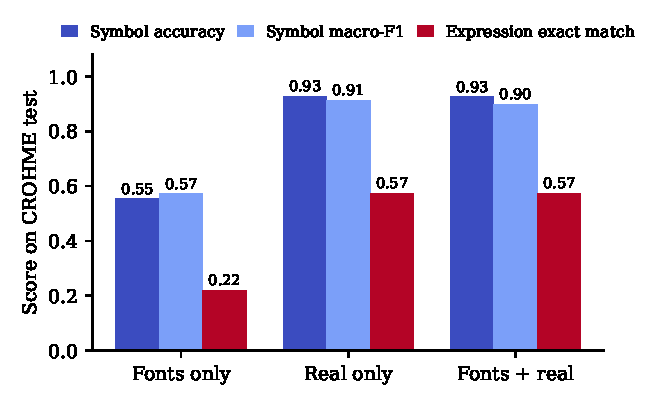
\includegraphics[width=\textwidth]{figures/fig_training_data.pdf}
\caption{Effect of training data on real-handwriting performance (same SVM).}\label{fig:traindata}
\end{minipage}\hfill
\begin{minipage}[t]{0.42\textwidth}\centering
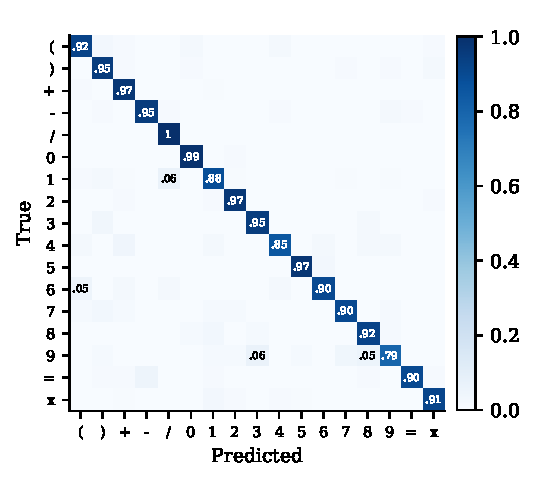
\includegraphics[width=\textwidth]{figures/fig_confusion_symbols.pdf}
\caption{Row-normalised confusion matrix on the CROHME test sets.}\label{fig:cm}
\end{minipage}
\end{figure}

\subsection{Comparison with a Deep-Learning OCR Baseline}

To test whether a lightweight classical model is competitive, we ran TrOCR~\cite{li2023trocr} (\texttt{trocr-base-handwritten}, 334M parameters) on the same 127 CROHME test expressions that fall within StepWise's symbol vocabulary. Each expression was cropped to its ink and passed to TrOCR as a text line. Because TrOCR was trained on general English handwriting, its output was normalised leniently before scoring: only digits and the seven operator symbols were kept, $\times$ was mapped to \texttt{x}, and spacing was made canonical. Table~\ref{tab:dl} shows that, without maths-specific fine-tuning, TrOCR read half as many expressions exactly as StepWise (McNemar test on exact matches: 40 vs.\ 4 expressions correct only for one system, $p=1.3\times10^{-7}$), while needing 28 times more time per expression on the same CPU and about 160 times more storage. TrOCR could be fine-tuned on CROHME, but that requires GPU training; the comparison shows that a classical pipeline trained on real data is a strong baseline for this restricted vocabulary.

\begin{table}[t]
\caption{StepWise vs.\ a zero-shot transformer OCR on 127 real CROHME test expressions (laptop CPU). 95\% bootstrap CIs in brackets.}\label{tab:dl}
\centering\small
\begin{tabular}{@{}lcccc@{}}
\toprule
System & Exact match & CER & ms/expr. & Size \\
\midrule
\textbf{StepWise (HOG + SVM)} & \textbf{0.567} [0.48, 0.65] & \textbf{0.115} & \textbf{48} & \textbf{8 MB} \\
TrOCR-base (zero-shot) & 0.284 [0.21, 0.36] & 0.369 & 1,325 & 1,336 MB \\
\bottomrule
\end{tabular}
\end{table}

\subsection{Robustness to Phone-Photo Conditions}

CROHME images are clean renderings, whereas students will photograph paper. We therefore degraded every test expression with Gaussian blur ($\sigma=1.5$), Gaussian noise ($\sigma=25$), JPEG compression (quality 20), a $5^\circ$ rotation, a horizontal lighting gradient, and a combination of rotation, lighting gradient, blur, noise and JPEG compression, and measured whole-expression accuracy with and without illumination normalisation (Table~\ref{tab:robust}). Blur, noise and compression had little effect, and rotation cost about eight points because the segmenter assumes horizontal lines. Uneven lighting was catastrophic for global thresholding (3.1\% exact) and was fully repaired by normalisation (56.7\%, identical to clean images). Under the combined photo-like degradation, normalisation raised exact match from 32.3\% to 51.2\% and cut the character error rate from 0.608 to 0.119. Clean-image accuracy was unchanged, so normalisation is enabled by default.

\begin{table}[t]
\caption{Whole-expression accuracy under simulated phone-photo degradations (127 CROHME test expressions), without and with illumination normalisation.}\label{tab:robust}
\centering\small
\begin{tabular}{@{}lcccc@{}}
\toprule
& \multicolumn{2}{c}{Exact match} & \multicolumn{2}{c}{CER} \\
\cmidrule(lr){2-3}\cmidrule(l){4-5}
Condition & without & with & without & with \\
\midrule
Clean & 0.567 & 0.567 & 0.115 & 0.115 \\
Blur & 0.559 & 0.559 & 0.114 & 0.113 \\
Noise & 0.575 & 0.575 & 0.119 & 0.119 \\
JPEG (q = 20) & 0.575 & 0.575 & 0.115 & 0.115 \\
Rotation $5^\circ$ & 0.488 & 0.480 & 0.131 & 0.133 \\
Uneven lighting & 0.031 & \textbf{0.567} & 0.528 & \textbf{0.115} \\
Combined photo-like & 0.323 & \textbf{0.512} & 0.608 & \textbf{0.119} \\
\bottomrule
\end{tabular}
\end{table}

\subsection{Misconception Diagnosis}

On the held-out 20\% of the generated solutions, the random forest reached a macro-F1 of 0.994, ahead of logistic regression (0.992), gradient boosting (0.991) and a depth-8 decision tree (0.979). The hand-written rule-based diagnoser that the system previously used reached only 0.330: it had zero recall for wrong operations, moving terms incorrectly and skipped steps, and it labelled incorrect algebra as correct whenever no answer key was given. Because the data are synthetic, these scores show that the features separate the modelled error types; they are not estimates of classroom accuracy.

Table~\ref{tab:real} reports the classifier trained on real mistakes (stratified 80/20 split, selection by 5-fold cross-validation on the training part). Distinguishing slips from understanding gaps is learnable from answer and scratchwork features: logistic regression reached 68.3\% accuracy (95\% CI 63.1--73.0\%) and an AUC of 0.76 (0.71--0.81), against 55.2\% for the majority class; the difference is significant (McNemar test, $p=9.4\times10^{-4}$). The seven-way task is harder because the categories overlap; the random forest reached 49.1\% accuracy (macro-F1 0.359) against 32.9\% for the majority baseline. Adding character n-grams of the Chinese question text raised the seven-class macro-F1 to 0.407, but that model cannot be applied to English questions and is reported only for reference. The most informative features were the digit edit distance between the answers, swapped answer blanks, the relative error and question length.

\begin{table}[t]
\caption{Error-type classification on ScratchMath (real student mistakes, held-out test set, $n=344$).}\label{tab:real}
\centering\small
\begin{tabular}{@{}lccc@{}}
\toprule
& \multicolumn{1}{c}{Slip vs.\ understanding} & \multicolumn{2}{c}{Seven error types} \\
\cmidrule(lr){2-2}\cmidrule(l){3-4}
Model & Accuracy (AUC) & Accuracy & Macro-F1 \\
\midrule
Majority baseline & 0.552 (--) & 0.329 & 0.071 \\
Random (stratified) baseline & 0.480 (--) & 0.267 & 0.161 \\
Logistic regression & \textbf{0.683} (0.765) & 0.340 & 0.307 \\
Random forest & 0.689 (0.772) & \textbf{0.491} & \textbf{0.359} \\
Gradient boosting & 0.704 (0.772) & 0.462 & 0.352 \\
\bottomrule
\end{tabular}
\end{table}

\begin{figure}[t]
\centering
\begin{minipage}[t]{0.52\textwidth}\centering
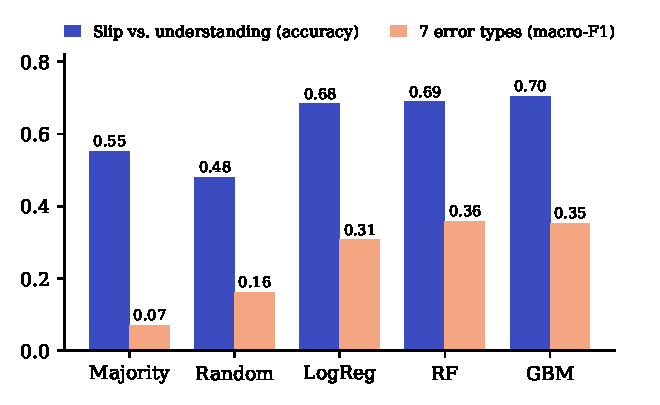
\includegraphics[width=\textwidth]{figures/fig_real_mistakes.pdf}
\caption{Real-mistake classifiers against baselines (ScratchMath).}\label{fig:realmis}
\end{minipage}\hfill
\begin{minipage}[t]{0.45\textwidth}\centering
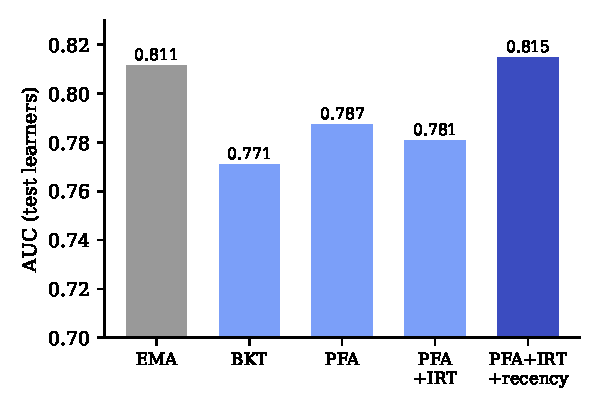
\includegraphics[width=\textwidth]{figures/fig_kt_auc.pdf}
\caption{Next-answer prediction on ASSISTments 2009 (test learners).}\label{fig:kt}
\end{minipage}
\end{figure}

\subsection{Knowledge Tracing}

On ASSISTments 2009 with a learner-disjoint 80/20 split (74,867 test answers), BKT fitted per skill by expectation--maximisation reached an AUC of 0.771 and PFA 0.787 (Fig.~\ref{fig:kt}). A simple exponential moving average of recent answers reached 0.811, reflecting a known property of this dataset: skill-builder problem sets end after a run of correct answers, so recent performance is highly predictive. Adding the recency features and Rasch item difficulty to PFA gave the highest AUC, 0.815 (95\% CI over learners 0.794--0.837), with the lowest root-mean-square error (0.396) and log-loss (0.476); the Rasch regularisation strength was chosen on validation learners. Its advantage over the moving average is not statistically significant (paired learner bootstrap: $+0.005$, 95\% CI $-0.017$ to $+0.024$), but it is clearly better than BKT, whose interval (0.744--0.802) lies almost entirely below it. StepWise uses BKT for the mastery display because its learned-state probability is directly interpretable by teachers. BKT parameters fitted on the matching ASSISTments skills are used for seven of StepWise's eight skills. In a simulation with 40 practice items per learner, choosing the least-mastered skill and items near 70\% predicted success left 74\% of skills learned, compared with 64\% for random or round-robin selection. On a simulated class with four planted groups, K-Means recovered the groups with an adjusted Rand index of 0.82.

\subsection{Ablation Studies}

Table~\ref{tab:ablation} removes feature groups from the two classifiers trained on real data. For symbols, HOG features carry almost all of the information (92.3\% accuracy alone, against 75.2\% for the zoning densities); zoning and the aspect ratio add little on top. For real mistakes, the answer-pattern features are the most useful single group, and removing them (question and image statistics only) costs 4.7 points of slip accuracy and 0.08 AUC. The scratchwork-image statistics improve the slip AUC (0.722 to 0.749) and the question statistics improve the seven-way accuracy (40.7\% to 49.1\%).

\begin{table}[t]
\caption{Feature ablations on held-out real data. Left: SVM symbol recognizer on CROHME test symbols. Right: ScratchMath slip-vs-understanding (logistic regression) and seven-type (random forest) classifiers.}\label{tab:ablation}
\centering\scriptsize
\begin{tabular}{@{}lcc@{\hspace{10pt}}lccc@{}}
\toprule
Symbol features & Acc. & F1 & Mistake features & Slip acc. & Slip AUC & 7-type acc. \\
\midrule
HOG only & 0.923 & 0.894 & Answer only & 0.657 & 0.722 & 0.407 \\
Zoning only & 0.752 & 0.746 & Answer + question & 0.677 & 0.757 & 0.491 \\
HOG + zoning & 0.925 & 0.898 & Answer + image & 0.663 & 0.749 & 0.424 \\
All (374) & 0.924 & 0.898 & Question + image & 0.637 & 0.683 & 0.378 \\
& & & All (42) & \textbf{0.683} & \textbf{0.765} & \textbf{0.491} \\
\bottomrule
\end{tabular}
\end{table}

\subsection{System Characteristics}

Fig.~\ref{fig:app} shows the student-facing analysis screen: each recognised symbol is drawn on the photograph and coloured by confidence, the first incorrect step is highlighted, and the diagnosis lists its supporting evidence alongside the real-data second opinion. All trained models together occupy about 25~MB. Processing one photograph took about 0.3~s on a laptop CPU (preprocessing 110~ms, recognition 11~ms, verification 97~ms, diagnosis 82~ms), with no network access. The backend is covered by 175 automated tests, and retraining every model from scratch with a fixed seed reproduces all reported numbers exactly.

\begin{figure}[t]
\centering
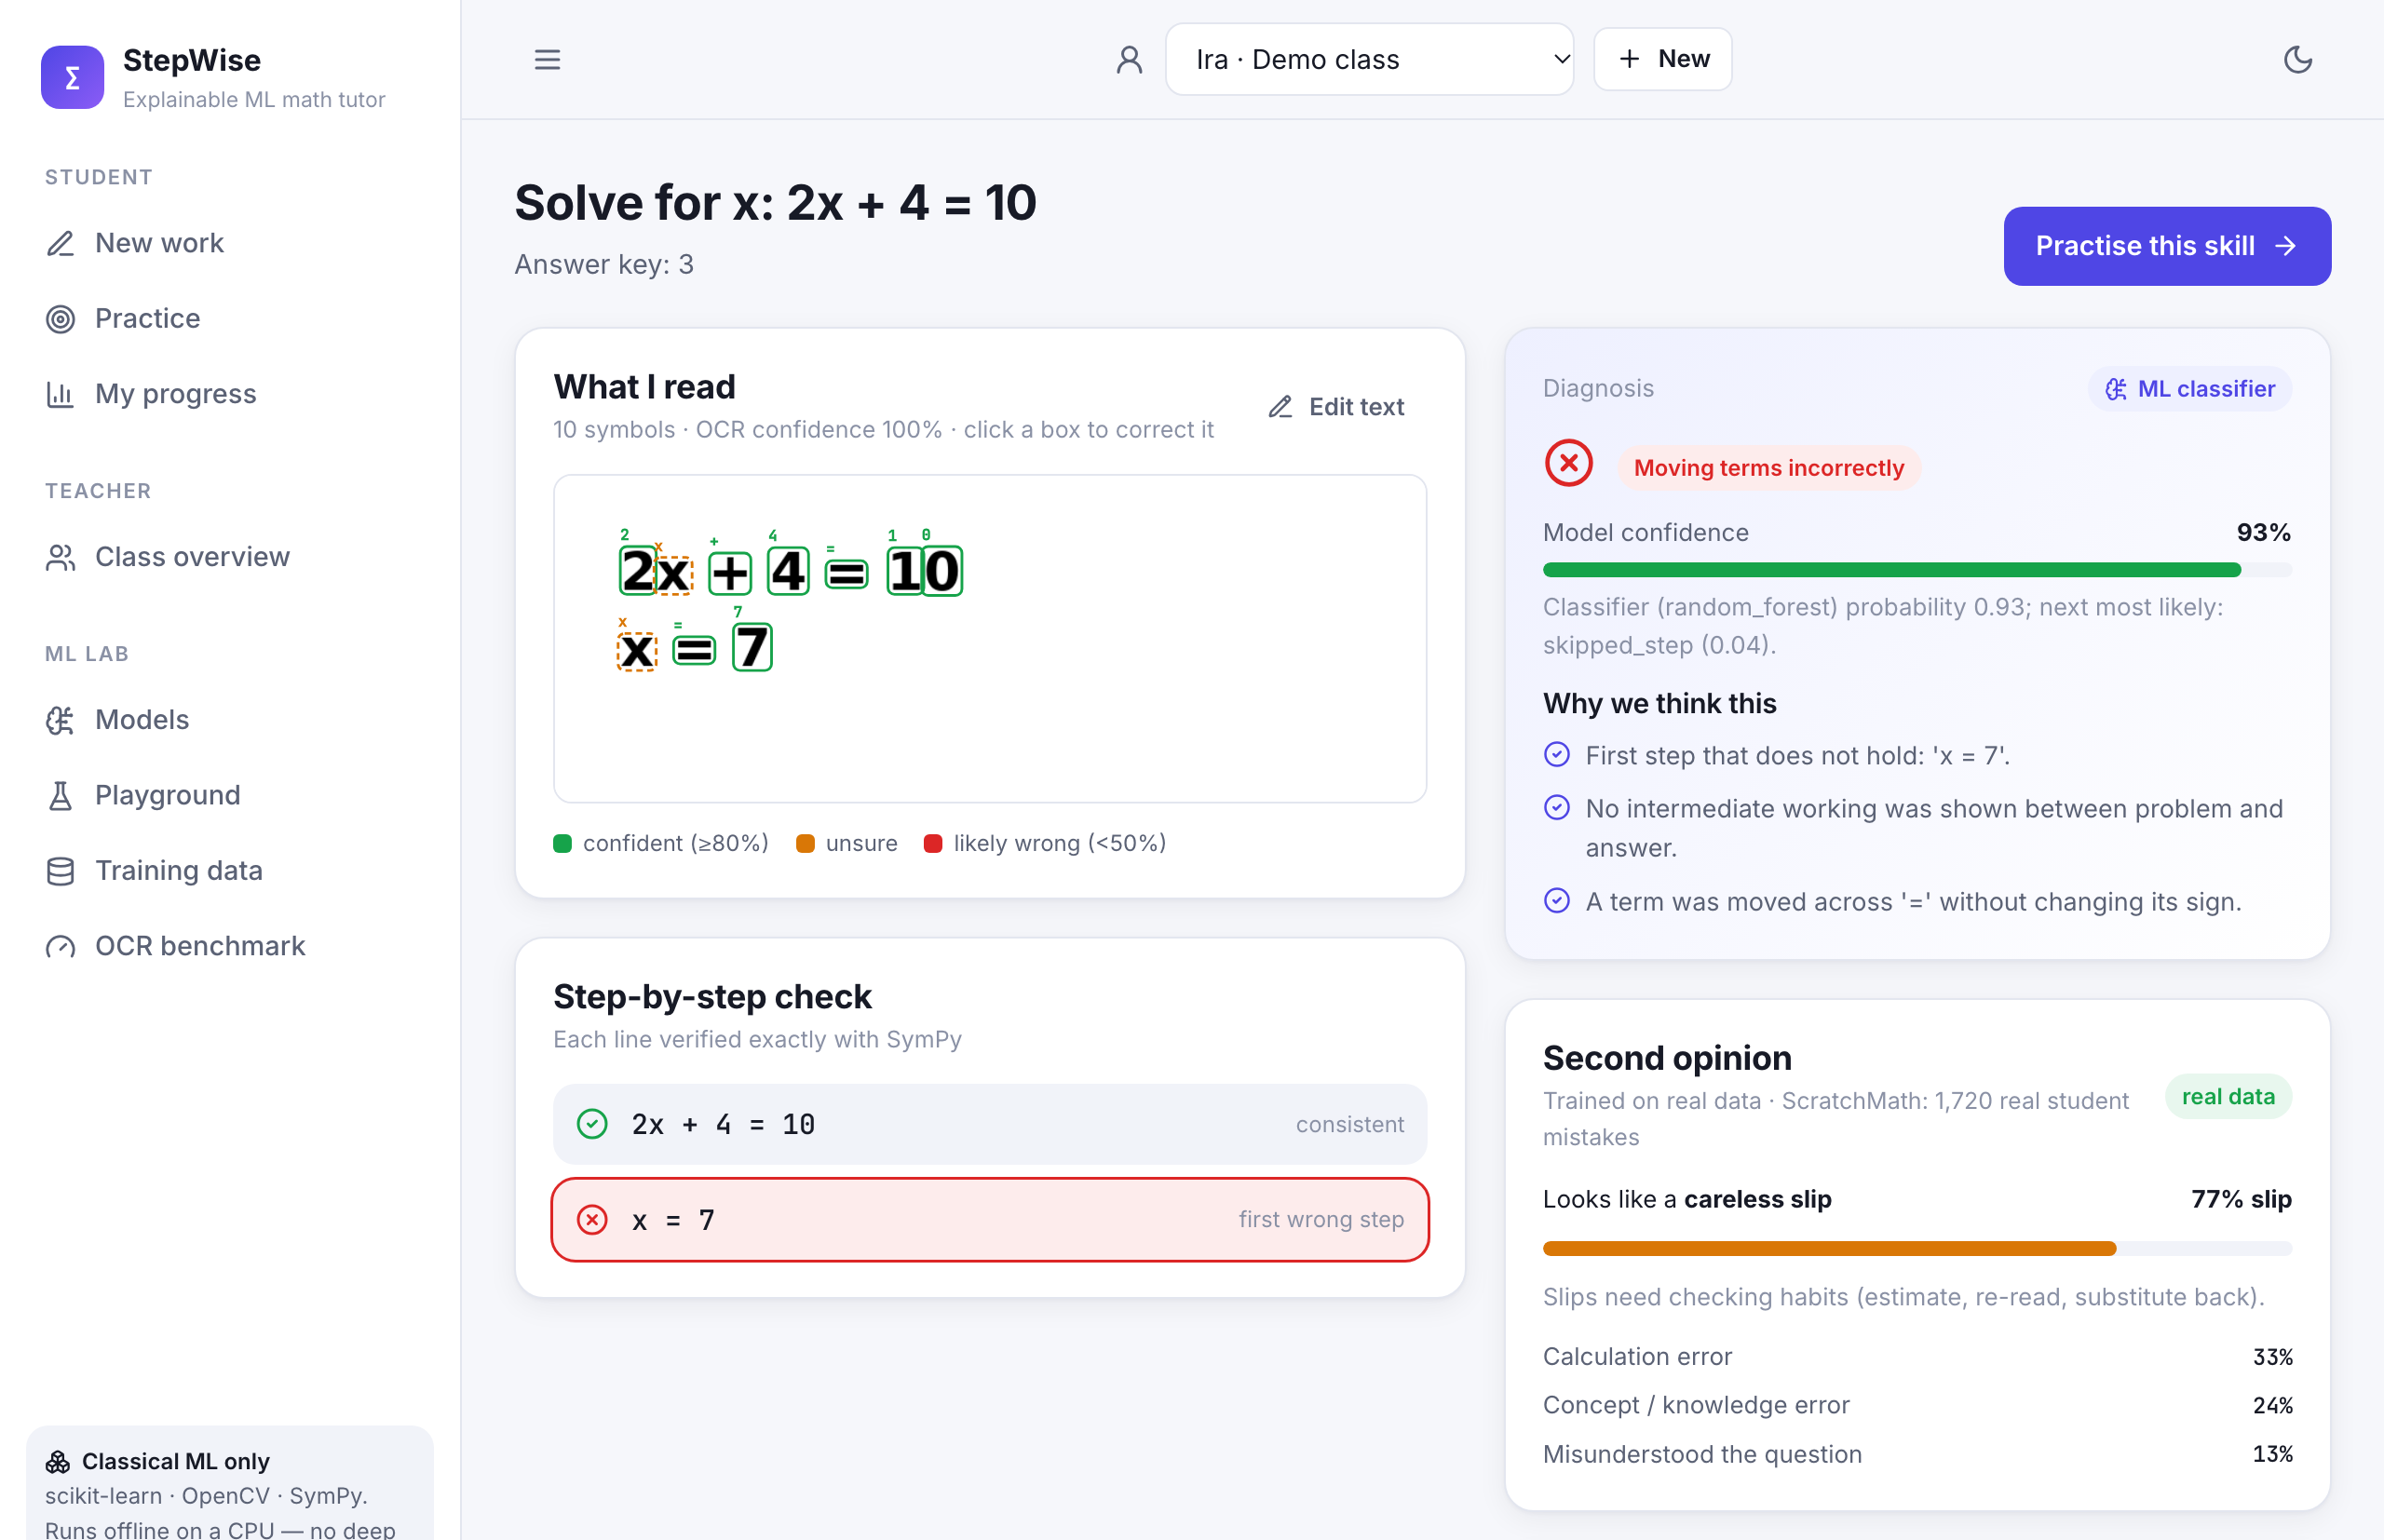
\includegraphics[width=\textwidth]{figures/fig_app_analysis.png}
\caption{Analysis screen: recognised symbols with confidence colours, step-by-step verification, the evidence-based diagnosis and the real-data second opinion.}\label{fig:app}
\end{figure}

\subsection{Limitations}

CROHME images are rendered from tablet handwriting rather than photographed paper; the degradation study approximates phone photographs, but real photographs of worksheets remain to be measured. Only linear expressions are harvested, and rotation beyond a few degrees still hurts segmentation. Count alignment can mislabel a crop when two segmentation errors cancel out. Segmentation assumes that symbols do not touch, so joined digits are not separated. The fine-grained misconception classifier is trained on generated data, and ScratchMath consists of Chinese word problems with a coarser label set. The adaptive-practice evaluation uses simulated learners.

%% ------------------------------------------------------------------
\section{Conclusion}

We presented StepWise, a tutoring system that reads handwritten mathematics, proves which step is wrong, explains the likely misconception and adapts practice, using only classical machine learning and exact symbolic computation. Training on real handwriting from CROHME and HASYv2 raised symbol accuracy on unseen writers from 55.4\% to 92.4\%, showing that synthetic font data alone is not a substitute for real writers. On the same real test expressions the classical recognizer read twice as many expressions exactly as a zero-shot transformer OCR model while being 28 times faster and 160 times smaller, and illumination normalisation made it robust to uneven lighting. On real student data, a classifier trained on 1,720 real mistakes separated careless slips from understanding gaps significantly better than chance (68.3\%), and knowledge tracing predicted next answers with an AUC of 0.815. The whole system is about 25~MB and runs offline on a CPU, which makes it suitable for classrooms without GPUs or reliable internet. Future work will collect and label photographs of English classroom worksheets to evaluate the fine-grained diagnosis on real data, fine-tune both recognizers on such photographs, and run a classroom pilot to measure learning gains.

%% ------------------------------------------------------------------
\begin{thebibliography}{99}

\bibitem{brown1978}
Brown JS, Burton RR (1978) Diagnostic models for procedural bugs in basic mathematical skills. Cognitive Science 2(2):155--192

\bibitem{koedinger1997}
Koedinger KR, Anderson JR, Hadley WH, Mark MA (1997) Intelligent tutoring goes to school in the big city. International Journal of Artificial Intelligence in Education 8:30--43

\bibitem{song2026scratchmath}
Song D, Xu T, Zhang YF, Li H, Yan Z, Fan X, Li H, Sun L, Wen Q (2026) Can MLLMs read students' minds? Unpacking multimodal error analysis in handwritten math. In: Proceedings of the 27th International Conference on Artificial Intelligence in Education (AIED)

\bibitem{vanlehn1990}
VanLehn K (1990) Mind bugs: the origins of procedural misconceptions. MIT Press, Cambridge, MA

\bibitem{mouchere2014}
Mouch\`ere H, Viard-Gaudin C, Zanibbi R, Garain U (2014) ICFHR 2014 competition on recognition of on-line handwritten mathematical expressions (CROHME 2014). In: 14th International Conference on Frontiers in Handwriting Recognition, pp 791--796

\bibitem{mahdavi2019}
Mahdavi M, Zanibbi R, Mouch\`ere H, Viard-Gaudin C, Garain U (2019) ICDAR 2019 CROHME + TFD: competition on recognition of handwritten mathematical expressions and typeset formula detection. In: International Conference on Document Analysis and Recognition, pp 1533--1538

\bibitem{zhang2017wap}
Zhang J, Du J, Zhang S, Liu D, Hu Y, Hu J, Wei S, Dai L (2017) Watch, attend and parse: an end-to-end neural network based approach to handwritten mathematical expression recognition. Pattern Recognition 71:196--206

\bibitem{li2023trocr}
Li M, Lv T, Chen J, Cui L, Lu Y, Florencio D, Zhang C, Li Z, Wei F (2023) TrOCR: transformer-based optical character recognition with pre-trained models. In: Proceedings of the AAAI Conference on Artificial Intelligence 37(11):13094--13102

\bibitem{dalal2005}
Dalal N, Triggs B (2005) Histograms of oriented gradients for human detection. In: IEEE Conference on Computer Vision and Pattern Recognition, pp 886--893

\bibitem{cortes1995}
Cortes C, Vapnik V (1995) Support-vector networks. Machine Learning 20(3):273--297

\bibitem{maji2009}
Maji S, Malik J (2009) Fast and accurate digit classification. Technical Report UCB/EECS-2009-159, University of California, Berkeley

\bibitem{thoma2017}
Thoma M (2017) The HASYv2 dataset. arXiv:1701.08380

\bibitem{corbett1994}
Corbett AT, Anderson JR (1994) Knowledge tracing: modeling the acquisition of procedural knowledge. User Modeling and User-Adapted Interaction 4(4):253--278

\bibitem{pavlik2009}
Pavlik PI, Cen H, Koedinger KR (2009) Performance factors analysis -- a new alternative to knowledge tracing. In: Artificial Intelligence in Education, pp 531--538

\bibitem{piech2015}
Piech C, Bassen J, Huang J, Ganguli S, Sahami M, Guibas LJ, Sohl-Dickstein J (2015) Deep knowledge tracing. In: Advances in Neural Information Processing Systems 28, pp 505--513

\bibitem{xiong2016}
Xiong X, Zhao S, Van Inwegen EG, Beck JE (2016) Going deeper with deep knowledge tracing. In: Proceedings of the 9th International Conference on Educational Data Mining, pp 545--550

\bibitem{rasch1960}
Rasch G (1960) Probabilistic models for some intelligence and attainment tests. Danish Institute for Educational Research, Copenhagen

\bibitem{feng2009}
Feng M, Heffernan N, Koedinger K (2009) Addressing the assessment challenge with an online system that tutors as it assesses. User Modeling and User-Adapted Interaction 19(3):243--266

\bibitem{meurer2017}
Meurer A, Smith CP, Paprocki M et al (2017) SymPy: symbolic computing in Python. PeerJ Computer Science 3:e103

\bibitem{breiman2001}
Breiman L (2001) Random forests. Machine Learning 45(1):5--32

\bibitem{pedregosa2011}
Pedregosa F, Varoquaux G, Gramfort A et al (2011) Scikit-learn: machine learning in Python. Journal of Machine Learning Research 12:2825--2830

\end{thebibliography}

\end{document}
